\hypertarget{particle_8h}{
\section{src/particle.h File Reference}
\label{particle_8h}\index{src/particle.h@{src/particle.h}}
}
Represents each of the finite charged particles. 

{\tt \#include $<$iostream$>$}\par


Include dependency graph for particle.h:\nopagebreak
\begin{figure}[H]
\begin{center}
\leavevmode
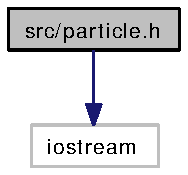
\includegraphics[width=63pt]{particle_8h__incl}
\end{center}
\end{figure}


This graph shows which files directly or indirectly include this file:\nopagebreak
\begin{figure}[H]
\begin{center}
\leavevmode
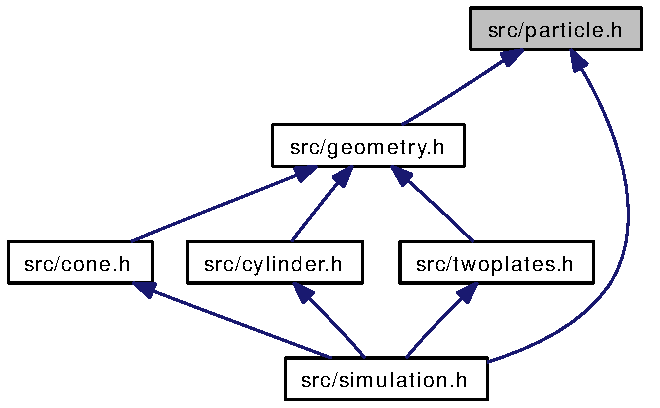
\includegraphics[width=176pt]{particle_8h__dep__incl}
\end{center}
\end{figure}
\subsection*{Classes}
\begin{CompactItemize}
\item 
class \hyperlink{classParticle}{Particle}
\end{CompactItemize}


\subsection{Detailed Description}
Represents each of the finite charged particles. 

Very basic class with stored the x-y position in the plane section and the energy of the particle.

\begin{Desc}
\item[Author:]Daniel Iglesias $<$\href{mailto:daniel.iglesias@ciemat.es}{\tt daniel.iglesias@ciemat.es}$>$ \end{Desc}
